\chapter{Почему суперсимметрия может быть важна}

\lectureoverview{Вакуумные флуктуации связывают темы этой главы.
Граничные условия порождают силу Казимира, петлевые эффекты ставят под угрозу массу Хиггса, новые виртуальные частицы изменяют бегущие калибровочные константы связи, а энергия вакуума управляет космическим расширением. Эти проблемы побуждают рассматривать низкоэнергетическую суперсимметрию как способ стабилизировать масштаб Хиггса, дать кандидата на тёмную материю и улучшить объединение калибровочных констант связи. Затем мы строим суперполя с помощью координат Грассмана и используем интегрирование Березина, чтобы извлечь суперсимметричное действие.}

\section{Вакуумные флуктуации между отражающими пластинами}

Мы возвращаемся к суперсимметрии, сначала разобрав один вопрос об эффекте Казимира. Поместим две параллельные отражающие пластины на расстоянии \(d\) друг от друга. Даже когда реальных частиц нет, квантовое поле обладает вакуумными флуктуациями. Их можно представлять как виртуальные процессы или, что эквивалентно, как нулевые колебания осцилляторных мод поля. Пластины задают граничные условия, поэтому допустимые между ними флуктуации отличаются от флуктуаций в неограниченном пространстве.

Важна не абсолютная нулевая точка энергии, а изменение, возникающее при изменении расстояния. Обозначим вакуумную энергию на единицу площади через \(\mathcal E(d)=E(d)/A\). Если \(\mathcal E\) зависит от \(d\), то это потенциальная энергия, и сила на единицу площади равна
\begin{equation}
\frac{F}{A}=-\frac{d\mathcal E}{dd}.
\end{equation}
Тем самым перестройка виртуальных процессов становится наблюдаемой силой. В привычном электромагнитном примере с идеальными проводящими пластинами энергия и давление равны
\begin{align}
\mathcal E(d)&=-\frac{\pi^2}{720\,d^3},\\
\frac{F}{A}&=-\frac{\pi^2}{240\,d^4},
\end{align}
в единицах \(\hbar=c=1\).\editorialnote{Эти коэффициенты и различие между энергией на единицу площади, убывающей как \(d^{-3}\), и давлением, убывающим как \(d^{-4}\), снимают вопрос о размерности, поднятый у доски. Это стандартный результат для идеальных пластин, а не вывод, выполняемый здесь.} Отрицательный знак означает притяжение.

\begin{classroomqa}
\audiencequestion{Относится ли четвёртая степень к силе или к энергии? \lecturetimestamp{00:04:39}}
\lecturerresponse{Для параллельных пластин в четырёхмерном пространстве-времени энергия на единицу площади убывает как \(d^{-3}\), тогда как дифференцирование по \(d\) даёт для силы на единицу площади зависимость \(d^{-4}\). Анализ размерностей уже фиксирует эти степени после восстановления \(\hbar\) и \(c\).}
\end{classroomqa}

Иногда это вычисление кратко излагают так: пластины прерывают петли виртуальных фотонов. Эта картина полезна, если не понимать её слишком буквально. Точное вычисление представляет собой изменение спектра допустимых мод поля или, что эквивалентно, изменение квантового эффективного действия. Оба языка приводят к одной и той же энергии, зависящей от расстояния.

\begin{classroomqa}
\audiencequestion{Может ли сила Казимира быть отталкивающей, а не притягивающей? \lecturetimestamp{00:07:48}}
\lecturerresponse{Может. Знак не универсален; он зависит от полей, геометрии, материалов и граничных условий. Фермионные петли часто дают знак, противоположный знаку бозонных петель, что и мотивирует высказанное у доски предположение, однако сама по себе фермионная статистика не является общей теоремой о том, что всякая сила Казимира должна быть отталкивающей.\editorialnote{Это уточнение заменяет намеренно осторожный ответ, данный в аудитории, общим утверждением, необходимым, чтобы избежать ложного универсального правила.}}
\end{classroomqa}

\subsection{Что можно было бы считать свидетельством энергии вакуума?}

Сила Казимира измерена, и атомные наблюдаемые тоже чувствительны к вакуумным петлям. Однако ни один из этих фактов сам по себе не доказывает, что абсолютная энергия вакуума гравитирует. Эксперимент по измерению силы Казимира измеряет разность энергий, вызванную границами; ту же силу можно описать и без приписывания операционального смысла неограниченной абсолютной сумме нулевых энергий.

Решающая проверка приходит со стороны гравитации. Энергия — это гравитационный заряд. Если пустое пространство несёт однородную плотность энергии, она должна входить в уравнения Эйнштейна и влиять на космическое расширение. Поэтому ускоренное расширение Вселенной является прямым гравитационным свидетельством вакуумоподобной компоненты.

\begin{classroomqa}
\audiencequestion{Почему в популярных изложениях энергию вакуума называют загадочной, будто физики не знают, что это такое? \lecturetimestamp{00:08:19}}
\lecturerresponse{Квантовая теория поля приписывает каждому полю вклад нулевой энергии, так что сама возможность энергии вакуума не является загадкой. Загадка носит количественный характер: почему гравитирующее значение настолько чрезвычайно мало по сравнению с оценками, основанными на известных квантовых полях и высокоэнергетическом обрезании? Поразителен не сам факт её наличия, а её почти полное отсутствие.}
\end{classroomqa}

В течение многих лет наблюдательный верхний предел был столь мал, что психологически возникал соблазн положить космологическую постоянную в точности равной нулю и искать принцип, который обеспечивал бы компенсацию. Но более точные космологические наблюдения обнаружили малое ненулевое значение. Это открытие не сделало энергию вакуума чем-то концептуально чуждым; оно сделало невозможным игнорировать необъяснённую степень подавления. Соответствующее сравнение зависит от предполагаемого ультрафиолетового масштаба, но всякая естественная высокоэнергетическая оценка требует колоссальной компенсации.

\section{Что один суперзаряд делает с многочастичным состоянием}

Прежде чем перечислять основания в пользу суперсимметрии, следует устранить возможный парадокс. Бозоны могут занимать одну моду в сколь угодно большом числе, тогда как фермионная мода имеет число заполнения 0 или 1. Если симметрия обменивает бозоны и фермионы, превращает ли она тысячу бозонов в одной моде в тысячу запрещённых фермионов?

Нет. Фермионный генератор изменяет по одному кванту за одно действие. В осцилляторной модели пусть \(a\) уничтожает бозон, а \(c^\dagger\) создаёт его фермионного партнёра. Один суперзаряд можно представить в виде
\begin{equation}
Q=c^\dagger a.
\end{equation}
На состоянии с \(n\) бозонами и без фермиона
\begin{equation}
Q\ket{n,0}
=\sqrt n\,\ket{n-1,1}.
\end{equation}
Один бозон уничтожен, и один фермион создан. Повторное действие тем же зарядом даёт нуль:
\begin{equation}
Q^2=(c^\dagger)^2a^2=0.
\end{equation}
Это нильпотентность, унаследованная от фермионных операторов рождения.

\begin{classroomqa}
\audiencequestion{Если много бозонов занимают одно и то же состояние, почему суперсимметричное преобразование не создаёт много фермионов в том же состоянии и не нарушает принцип запрета? \lecturetimestamp{00:12:05}}
\lecturerresponse{Генератор не заменяет сразу всё заполнение. Он изменяет состояние на одну единицу фермионного числа. Один и тот же фермионный заряд нельзя комбинировать, как обычный генератор вращения, потому что его квадрат равен нулю. Другой, дополняющий его, заряд может обратить этот обмен, а смешанный антикоммутатор замыкается на перенос по времени.}
\end{classroomqa}

Последнее предложение существенно. Сокращённая запись \(Q^2=0\) относится к отдельной хиральной компоненте или к простому заряду, который только что был выписан; она не означает, что любое произведение суперзарядов обращается в нуль. В четырёхмерной суперсимметрии,
\begin{equation}
\{Q_\alpha,\bar Q_{\dot\beta}\}
=2\sigma^\mu_{\alpha\dot\beta}P_\mu,
\end{equation}
тогда как
\begin{equation}
\{Q_\alpha,Q_\beta\}=0,
\qquad
\{\bar Q_{\dot\alpha},\bar Q_{\dot\beta}\}=0
\end{equation}
в минимальной алгебре без центральных зарядов.\editorialnote{Эта запись по компонентам уточняет сокращённую аудиторную формулировку: повторное действие одного и того же \(Q\) даёт нуль, тогда как суперзаряд и его сопряжённый порождают трансляцию.}

\section{Три причины искать низкоэнергетическую суперсимметрию}

\begin{classroomqa}
\audiencequestion{Есть ли мотивация для суперсимметрии помимо компенсации энергии вакуума? \lecturetimestamp{00:15:06}}
\lecturerresponse{Есть три тесно связанные мотивации: контроль над самоэнергией Хиггса, возможная стабильная частица тёмной материи и гораздо более точное схождение калибровочных констант связи при высоких энергиях. Ни одна из них не доказывает, что суперсимметрия реализована в природе, но вместе они делают её серьёзной теорией, которую стоит проверять.}
\end{classroomqa}

Выражение \emph{низкоэнергетическая суперсимметрия} относительно. Оно не означает, что суперпартнёры легки в обыденном смысле; оно означает, что их массы не находятся намного выше электрослабого масштаба и масштабов ускорителей. Все три аргумента ослабевают, если суперпартнёров поднять на сколь угодно высокие массы.

\subsection{Защита масштаба Хиггса}

Масса скаляра необычно чувствительна к высокоэнергетической физике. Схематически бозонная петля даёт поправку вида
\begin{equation}
\delta m_H^2\big|_{\mathrm B}
\sim +\frac{\lambda}{16\pi^2}\Lambda^2,
\end{equation}
где \(\Lambda\) обозначает масштаб, до которого применяется эффективная теория. Фермионная петля даёт вклад противоположного знака,
\begin{equation}
\delta m_H^2\big|_{\mathrm F}
\sim -\frac{|y|^2}{8\pi^2}\Lambda^2.
\end{equation}
Коэффициенты зависят от взаимодействия и кратностей полей, однако суперсимметрия связывает их так, что ведущая ультрафиолетовая чувствительность взаимно сокращается между партнёрами.\editorialnote{Эти схематические петлевые формулы показывают математику, стоящую за качественным аргументом о самоэнергии. Они не предназначены служить полным расчётом массы Хиггса в Стандартной модели.}

Это важно потому, что среднее значение поля Хиггса задаёт электрослабый масштаб. Массы калибровочных бозонов и фермионов подчиняются таким соотношениям, как
\begin{equation}
m_W=\frac{gv}{2},
\qquad
m_f=\frac{y_fv}{\sqrt2}.
\end{equation}
Если бы сектор Хиггса естественным образом уводился на огромный масштаб, привычный низкоэнергетический спектр частиц был бы утрачен, если только голые параметры не были бы подогнаны в компенсацию радиационных поправок с чрезвычайной точностью.

Точная суперсимметрия делала бы эту компенсацию точной, но точная суперсимметрия уже исключена неравенством масс наблюдаемых бозонов и фермионов. При мягко нарушенной суперсимметрии квадратичная чувствительность заменяется зависимостью от расщеплений суперпартнёров; схематически
\begin{equation}
\delta m_H^2
\sim
\frac{g^2}{16\pi^2}
\left(m_{\mathrm{soft}}^2-m_{\mathrm{ordinary}}^2\right)
\ln\frac{\Lambda^2}{m_{\mathrm{soft}}^2}.
\end{equation}
Эта компенсация остаётся полезной лишь до тех пор, пока расщепление не слишком велико.

\subsection{Стабильный конечный продукт каскадов тёмной материи}

Разделим спектр на обычные частицы и их суперпартнёров. У фермиона есть бозонный партнёр; у бозона — фермионный. Если взаимодействия сохраняют чётность, различающую эти два класса, то распад суперпартнёра должен оставлять ещё одного суперпартнёра:
\begin{equation}
\widetilde X
\longrightarrow X+\widetilde Y
\longrightarrow X+Y+\widetilde Z
\longrightarrow\cdots.
\end{equation}
Каскад не может избавиться от своего последнего суперпартнёра. Поэтому он заканчивается на самой лёгкой суперсимметричной частице, LSP.

Обычно используемая симметрия — \(R\)-чётность,
\begin{equation}
R_p=(-1)^{3(B-L)+2s}.
\end{equation}
Частицы Стандартной модели имеют \(R_p=+1\), тогда как их суперпартнёры — \(R_p=-1\). Если \(R_p\) точна, каждое взаимодействие содержит чётное число суперпартнёров, и LSP стабильна.\editorialnote{Сама по себе суперсимметрия не гарантирует стабильности LSP. Для стабильности требуется сохраняемая \(R\)-чётность или другая симметрия с тем же следствием; без неё LSP может распадаться.}

Тёмная материя должна сохраняться по меньшей мере в течение космологических времён. Она также должна взаимодействовать достаточно слабо, чтобы многократно проходить через видимый галактический диск, не теряя существенной энергии. Электрически заряженная или сильно взаимодействующая популяция рассеивалась бы, диссипировала энергию и имела бы тенденцию коллапсировать к той же тонкой структуре, что и обычное вещество. Наблюдаемое протяжённое гало, напротив, указывает на нейтральную, слабо взаимодействующую компоненту.

Это не определяет LSP однозначно. В зависимости от модели и схемы нарушения симметрии кандидатом может быть нейтральная смесь электрослабых гаугино и хиггсино, или же гравитино. Заряженные или цветные кандидаты жёстко ограничены. Суперсимметрия даёт не гарантированный ответ, а естественный механизм, приводящий к нейтральному долгоживущему конечному продукту.

\section{Бегущие константы связи и намёк на объединение}

Третья мотивация начинается с экранирования заряда. Измеряемая константа связи зависит от энергетического масштаба, потому что виртуальные частицы одевают взаимодействие. В электромагнетизме электрон-позитронная петля, вставленная в пропагатор фотона, экранирует заряд на больших расстояниях. На меньших расстояниях, или при большем переданном импульсе, меньшая часть этого поляризационного облака оказывается между пробными частицами, и эффективный заряд больше.

Запишем
\begin{equation}
\alpha_i=\frac{g_i^2}{4\pi}.
\end{equation}
На однопетлевом уровне обратная константа связи меняется линейно с логарифмом энергии:
\begin{equation}
\frac{d\alpha_i^{-1}}{d\ln\mu}
=-\frac{b_i}{2\pi}.
\end{equation}
Таким образом,
\begin{equation}
\alpha_i^{-1}(\mu)
=\alpha_i^{-1}(\mu_0)
-\frac{b_i}{2\pi}\ln\frac{\mu}{\mu_0}.
\end{equation}
\editorialnote{Это однопетлевое уравнение — точная версия почти прямых линий, рисуемых как функции логарифма энергии. Пороги и многопетлевые поправки слегка искривляют эти линии.}

Выше электрослабого масштаба тремя фундаментальными калибровочными константами связи являются константы групп
\begin{equation}
U(1)_Y,\qquad SU(2)_L,\qquad SU(3)_c.
\end{equation}
Электромагнитная константа связи, которой удобно пользоваться для интуиции при низких энергиях, после электрослабого нарушения симметрии представляет собой комбинацию первых двух. В КХД неабелевы калибровочные поля вызывают антиэкранирование: сильная константа связи уменьшается на малых расстояниях — это явление асимптотической свободы. Поэтому \(\alpha_3^{-1}\) растёт с \(\ln\mu\), тогда как остальные обратные константы связи имеют другие наклоны.

Кривые Стандартной модели, по-видимому, тяготеют друг к другу, но не сходятся в одной точке. Суперпартнёры модифицируют виртуальные петли и тем самым изменяют коэффициенты \(b_i\). В обычной нормировке великого объединения,
\begin{align}
(b_1,b_2,b_3)_{\mathrm{SM}}
&=\left(\frac{41}{10},-\frac{19}{6},-7\right),\\
(b_1,b_2,b_3)_{\mathrm{MSSM}}
&=\left(\frac{33}{5},1,-3\right).
\end{align}
При порогах суперпартнёров вблизи масштаба TeV экстраполированные суперсимметричные кривые сходятся гораздо точнее вблизи
\begin{equation}
M_{\mathrm{GUT}}\sim 10^{16}\ \mathrm{GeV}.
\end{equation}
Ни один эксперимент напрямую не достигает этого масштаба. Низкоэнергетические константы связи измеряются, полевое содержание определяет бег, и кривые экстраполируются на многие порядки по энергии. Две линии всегда где-нибудь пересекутся; нетривиально то, что три независимые линии сходятся почти в одной точке.

\begin{classroomqa}
\audiencequestion{Предполагает ли улучшенная экстраполяция точную суперсимметрию и равенство масс партнёров? \lecturetimestamp{00:38:09}}
\lecturerresponse{Нет. Суперсимметрия нарушена, поэтому массы расщеплены. Важно то, на каком масштабе петли суперпартнёров начинают вносить вклад в бег. Если партнёры не слишком тяжелы, наклоны меняются достаточно рано, чтобы три константы связи сошлись. Если же они чрезвычайно тяжелы, суперсимметричные пороги появляются слишком поздно, и улучшенное схождение теряется.}
\end{classroomqa}

Пороговые поправки и неизвестный высокоэнергетический спектр не позволяют в буквальном смысле утверждать, что три линии сходятся с математической точностью. Тем не менее результат поразителен: тот же приблизительный масштаб суперпартнёров, который помогает Хиггсу и даёт термального кандидата тёмной материи, также улучшает объединение.

\subsection{Гравитация и общий высокоэнергетический масштаб}

Гравитация ведёт себя иначе, потому что её зарядом является сама энергия. Удобной безразмерной мерой при энергии в системе центра масс \(E\) служит
\begin{equation}
\alpha_G(E)\sim GE^2
=\left(\frac{E}{M_{\mathrm{Pl}}}\right)^2.
\end{equation}
При обычных энергиях эта величина фантастически мала, но растёт квадратично с \(E\). Поэтому её обратная величина убывает гораздо быстрее, чем логарифмически бегущие обратные калибровочные константы связи, и становится порядка единицы вблизи планковского масштаба.

Это сравнение наводит на мысль, что все взаимодействия могут определяться близкими высокими масштабами, но оно менее прозрачно, чем калибровочное объединение. Калибровочные константы связи — безразмерные параметры в перенормируемых теориях поля; постоянная Ньютона размерна, поэтому для нанесения гравитации на тот же график требуется соглашение.

\begin{classroomqa}
\audiencequestion{Участвуют ли суперпартнёры в тех же трёх калибровочных взаимодействиях, или они определяют новые силы? \lecturetimestamp{00:42:35}}
\lecturerresponse{Они несут те же калибровочные квантовые числа, что и их партнёры. Селектрон имеет электрический заряд электрона, а скварк — цвет и электрослабые заряды соответствующего кварка, хотя их спины и массы различаются. Поэтому их петли модифицируют те же калибровочные взаимодействия, а не вводят три новых.}
\end{classroomqa}

\begin{classroomqa}
\audiencequestion{Было бы открытие суперпартнёра на LHC окончательным свидетельством суперсимметрии? \lecturetimestamp{00:43:27}}
\lecturerresponse{Одной незнакомой частицы было бы недостаточно, если судить лишь по названию, но спектр суперпартнёров, подчиняющийся суперсимметричным соотношениям между спинами, зарядами, массами и константами связи, был бы весьма характерен. Суперсимметрия накладывает много взаимосвязанных ограничений, поэтому детальная картина взаимодействий дала бы решающий тест.}
\end{classroomqa}

\subsection{Почему этот масштаб нельзя отодвинуть без потерь}

Если суперпартнёры лежат лишь немного за пределами экспериментальной досягаемости, все три мотивации ещё могут работать. Если их массы повысить на много порядков, каждый аргумент слабеет:
\begin{enumerate}
\item Компенсации в массе Хиггса оставляют большую остаточную чувствительность к расщеплению.
\item Обычный термальный реликт слабого масштаба больше не возникает на ожидаемом масштабе.
\item Пороги бега калибровочных констант связи смещаются вверх, и три константы связи сходятся менее точно.
\end{enumerate}
Суперсимметрия всё ещё могла бы существовать на гораздо более высоком масштабе, но тогда она уже не решала бы эти конкретные низкоэнергетические проблемы столь же экономным способом. Долговечность этой идеи не является доказательством того, что природа обязана её использовать; она лишь показывает, что предложение достаточно непротиворечиво, чтобы заслуживать решающего теста.

\section{Что космология может и чего не может сказать нам о тёмной материи}

\begin{classroomqa}
\audiencequestion{Может ли стандартная космология определить количество тёмной материи и массу каждой частицы тёмной материи, подобно тому как нуклеосинтез накладывает ограничения на водород и гелий? \lecturetimestamp{00:46:32}}
\lecturerresponse{Космология очень хорошо измеряет полную массовую плотность тёмной материи, но одна лишь плотность не отделяет массу от числа. Одна и та же плотность может обеспечиваться небольшим числом тяжёлых частиц или огромным числом очень лёгких. Чтобы установить, какая именно микроскопическая частица стоит за этим, нужны дополнительная теория или негравитационные наблюдения.}
\end{classroomqa}

Эту неоднозначность иллюстрируют два широких класса возможностей. Слабо взаимодействующая частица вблизи электрослабого масштаба или масштаба TeV может вымерзнуть из горячей тепловой бани. На другом конце чрезвычайно лёгкий бозон, такой как аксион, может находиться в когерентной конфигурации поля или в конденсате. Промежуточные возможности не запрещены лишь потому, что два наиболее разработанных механизма расположены у противоположных концов.

Сама структура гало даёт важное ограничение. Тёмная материя проходит сквозь обычное вещество с малым трением, поэтому она остаётся пространственно протяжённой, а не коллапсирует в светящийся диск. Кривые вращения и другие гравитационные явления говорят нам, что эта масса присутствует, но сами по себе они не подсчитывают число частиц.

\begin{classroomqa}
\audiencequestion{Могла ли ранняя Вселенная первоначально содержать только суперчастицы, которые позднее распались на наблюдаемые нами частицы? \lecturetimestamp{00:49:11}}
\lecturerresponse{При температурах, намного превышающих все существенные массы, быстрые реакции приводят разные виды частиц к тепловому равновесию, а не к произвольной односторонней населённости. Обычные столкновения рождают суперпартнёров, когда тех недостаёт, тогда как столкновения и распады суперпартнёров пополняют число обычных частиц. Точное содержание зависит от взаимодействий и числа степеней свободы, но горячая плазма непрерывно стремится к балансу.}
\end{classroomqa}

По мере остывания Вселенной массивные виды испытывают больцмановское подавление и аннигилируют или распадаются. Стабильная LSP перестаёт отслеживать равновесное содержание, когда скорость её взаимодействия становится меньше скорости космического расширения:
\begin{equation}
\Gamma_{\mathrm{ann}}
\sim n\langle\sigma v\rangle
\lesssim H.
\end{equation}
Оставшиеся частицы образуют реликтовое обилие.\editorialnote{Этот критерий вымораживания является стандартным количественным завершением аргумента о тепловом балансе. У других кандидатов на роль LSP, особенно у очень слабо взаимодействующих гравитино, возможна нетепловая история.}

\begin{classroomqa}
\audiencequestion{Суперпартнёром какой обычной частицы является LSP, и обязана ли она вообще не взаимодействовать? \lecturetimestamp{00:51:05}}
\lecturerresponse{Модельно-независимого ответа нет. Ожидается, что LSP, пригодная на роль тёмной материи, электрически нейтральна и бесцветна, но она не обязана быть полностью невзаимодействующей. Она может быть смесью состояний, связанных с фотоном, слабыми калибровочными бозонами и полями Хиггса, или же это может быть гравитино. Её точная природа определяется спектром нарушения суперсимметрии.}
\end{classroomqa}

\section{Вакуумные диаграммы, диаграммы самоэнергии и расширение}

\begin{classroomqa}
\audiencequestion{В чём различие между расходимостью Хиггса и расходимостью вакуумной энергии? \lecturetimestamp{00:52:09}}
\lecturerresponse{У вакуумной диаграммы нет внешних линий частиц; она изменяет эффективное действие пустого пространства и вносит вклад в вакуумную энергию. Диаграмма самоэнергии Хиггса имеет две внешние ножки Хиггса; она изменяет пропагатор Хиггса и, следовательно, его массу. Обе связаны с виртуальными флуктуациями, но отвечают на разные вопросы.}
\end{classroomqa}

Можно представить себе реальную частицу как примесь, внесённую в вакуум. Вакуумные флуктуации, присоединяющиеся к этой примеси, смещают её распространение и массу. Пластины Казимира тоже изменяют вакуумные флуктуации, но за счёт макроскопических граничных условий. Общее здесь — отклик квантовых флуктуаций на то, что было внесено; однако корректируемая наблюдаемая величина в каждом случае различна.

\vspace{-2pt}
\subsection{Вещество, излучение и вакуум разрежаются по-разному}

Пусть \(a(t)\) — космологический масштабный фактор, а
\begin{equation}
H=\frac{\dot a}{a}
\end{equation}
— параметр Хаббла. Локальное сохранение тензора энергии-импульса в однородной Вселенной даёт
\begin{equation}
\dot\rho+3H(\rho+p)=0.
\end{equation}
Для уравнения состояния \(p=w\rho\) отсюда следует
\begin{equation}
\rho(a)\propto a^{-3(1+w)}.
\end{equation}
\editorialnote{Уравнение непрерывности даёт компактный вывод, лежащий в основе объяснений через подсчёт частиц и растяжение длины волны.}

Для холодного нерелятивистского вещества \(p\approx0\), поэтому
\begin{equation}
\rho_m\propto a^{-3}.
\end{equation}
Фиксированный сопутствующий объём растёт как \(a^3\), тогда как энергия покоя, переносимая его частицами, остаётся приблизительно постоянной.

Для излучения \(p=\rho/3\), и
\begin{equation}
\rho_r\propto a^{-4}.
\end{equation}
Три степени связаны с разрежением числовой плотности. Четвёртая — с красным смещением:
\begin{equation}
\lambda\propto a,
\qquad
E_\gamma=\frac{2\pi\hbar c}{\lambda}\propto a^{-1}.
\end{equation}

\begin{classroomqa}
\audiencequestion{Если у фотона есть волновая функция, почему при выводе закона разрежения можно говорить о нём как о частице, а не как о волне? \lecturetimestamp{00:58:21}}
\lecturerresponse{Это различие не влияет на закон масштабирования. В описании через частицы число квантов в сопутствующем объёме фиксировано, и каждый квант испытывает красное смещение так, что его энергия ведёт себя как \(a^{-1}\). В описании через классическую волну длина волны растягивается, и энергия поля падает на ту же величину. Можно пользоваться тем языком, в котором расширение легче всего увидеть.}
\end{classroomqa}

Для вакуумной энергии \(p_\Lambda=-\rho_\Lambda\), поэтому
\begin{equation}
\rho_\Lambda=\text{constant}.
\end{equation}
Она не разрежается при расширении пространства. Действительно, в сопутствующей области содержится
\begin{equation}
E_\Lambda=\rho_\Lambda a^3V_0,
\end{equation}
и эта величина растёт вместе с её физическим объёмом. Этот факт порождает вопрос о сохранении энергии, к которому мы вскоре вернёмся.

Эти разные степени определяют ход космической истории. Излучение убывает быстрее всего, вещество — медленнее, а вакуумная энергия не убывает вовсе. Поэтому даже очень малый вакуумный член может быть пренебрежимо малым в ранней Вселенной и доминировать в поздние времена. Используя обсуждавшиеся здесь грубые оценки, получаем, что современный энергетический бюджет составляет примерно \(70\%\) вакуумной энергии и \(30\%\) вещества, причём вклад излучения намного меньше.

\section{Геометрия равна энергии}

Компонента время–время уравнений Эйнштейна превращает предыдущие законы масштабирования в динамику. На доске всё начинается с лозунга и одного геометрического члена.

\begin{figure}[H]
\centering
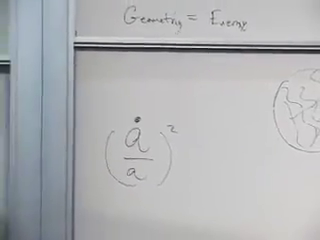
\includegraphics[width=0.68\textwidth]{lecture_06_figure_03.png}
\lectureframe{01:06:37.088}
\caption{Организующий лозунг \emph{геометрия равна энергии}, а под ним записан член расширения \(H^2=(\dot a/a)^2\).}
\end{figure}

Для однородной и изотропной Вселенной первое уравнение Фридмана имеет вид
\begin{equation}
H^2+\frac{k}{a^2}
=\frac{8\pi G}{3}\rho,
\end{equation}
в единицах \(c=1\), где \(k=+1,0,-1\) обозначает соответственно замкнутую, плоскую или открытую пространственную геометрию, а полная плотность энергии равна
\begin{equation}
\rho
=\rho_{\mathrm{ordinary}}
+\rho_{\mathrm{dark}}
+\rho_{\mathrm{radiation}}
+\rho_{\mathrm{vacuum}}.
\end{equation}
Знак, стоящий рядом с \(1/a^2\), зависит от того, оставляют ли член кривизны слева или переносят вправо, а также от значения \(k\).

\begin{figure}[H]
\centering
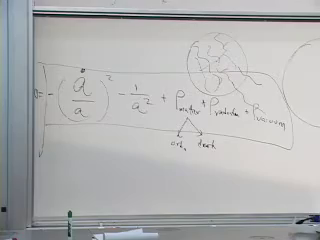
\includegraphics[width=0.96\textwidth]{lecture_06_figure_04.png}
\lectureframe{01:08:46.794}
\caption{Полный баланс на доске: расширение и пространственная кривизна на геометрической стороне, а вещество, излучение и вакуумная энергия — на стороне источников. Вещество далее разделено на обычную и тёмную компоненты.}
\end{figure}

\subsection{Космологическое гамильтоново ограничение}

\begin{classroomqa}
\audiencequestion{Если вакуумная энергия в сопутствующей области растёт по мере расширения Вселенной, существует ли тогда постоянная суммарная плотность энергии или сохраняется полная энергия? \lecturetimestamp{01:01:51}}
\lecturerresponse{Общая теория относительности не задаёт универсальной глобальной энергии для произвольного расширяющегося пространства-времени. Однако в однородной космологической редукции уравнение Эйнштейна для компоненты время–время является гамильтоновым ограничением. Если геометрические и материальные члены собрать в одной части уравнения, гамильтониан с ограничением обращается в нуль. Меняющиеся члены материи уравновешиваются гравитационными степенями свободы, а не обычной фиксированной энергией в ящике.}
\end{classroomqa}

Схематически каноническое утверждение имеет вид
\begin{equation}
\mathcal H_{\mathrm{gravity}}
+\mathcal H_{\mathrm{matter}}
=0.
\end{equation}
Именно в этом состоит точный смысл утверждения, что полная энергия равна нулю. Это уравнение движения, навязываемое инвариантностью относительно перепараметризации времени, а не утверждение о том, что всякая локальная плотность энергии обращается в нуль. В сопутствующем объёме энергия обычного вещества приблизительно постоянна, энергия излучения уменьшается, а вакуумная энергия растёт; тем временем гравитационный вклад и скорость расширения подстраиваются так, чтобы ограничение Эйнштейна продолжало выполняться.

Локальное сохранение остаётся точным:
\begin{equation}
\nabla_\mu T^{\mu\nu}=0.
\end{equation}
Для однородного флюида это в точности уравнение непрерывности \(\dot\rho+3H(\rho+p)=0\). Обычно неверна интуиция плоского пространства-времени, согласно которой в расширяющейся Вселенной должна существовать и одна координатно-независимая глобальная сумма энергии материи, сохраняющаяся во времени.\editorialnote{Это различие делает точным утверждение, прозвучавшее на лекции, что энергия всегда равна нулю: локальное ковариантное сохранение и космологическое гамильтоново ограничение точны, тогда как однозначно определённая глобальная энергия материи и гравитации, вообще говоря, не определена.}

\begin{classroomqa}
\audiencequestion{Является ли нулевое ограничение условием, определяющим, открыта Вселенная, замкнута или плоска? \lecturetimestamp{01:04:42}}
\lecturerresponse{Нет. Гамильтоново ограничение действует во всех случаях. Открытые, плоские и замкнутые вселенные различаются меткой кривизны \(k\) и, следовательно, членом \(k/a^2\). Кривизна изменяет один из вкладов в баланс; она не включает и не выключает ограничение.}
\end{classroomqa}

\section{Координаты Грассмана и суперполя}

\begin{classroomqa}
\audiencequestion{Возникают ли числа Грассмана непосредственно в лагранжиане теории? \lecturetimestamp{01:09:37}}
\lecturerresponse{Сначала они возникают потому, что фермионные поля грассманово нечётны. Затем — как координаты суперпространства. Суперполя зависят от этих нечётных координат, а суперсимметричные действия строятся дифференцированием и интегрированием по ним.}
\end{classroomqa}

Обычное поле является функцией пространства-времени,
\begin{equation}
\phi=\phi(x^\mu).
\end{equation}
Минимальная суперсимметрия в четырёх измерениях дополняет \(x^\mu\) двухкомпонентным нечётным спинором \(\theta^\alpha\) и сопряжённым к нему \(\bar\theta^{\dot\alpha}\):
\begin{equation}
z^M=(x^\mu,\theta^\alpha,\bar\theta^{\dot\alpha}).
\end{equation}
Имеются две комплексные нечётные компоненты, или 4 вещественных нечётных направления. Суперполе — это функция на этом суперпространстве:
\begin{equation}
\Phi=\Phi(x,\theta,\bar\theta).
\end{equation}

Это не крошечные пространственные измерения в метрическом смысле. Координата Грассмана не имеет положительной численной величины. Называть её малой — лишь мнемоника для нильпотентности:
\begin{equation}
(\theta^\alpha)^2=0,
\qquad
\theta^\alpha\theta^\beta=-\theta^\beta\theta^\alpha.
\end{equation}
\editorialnote{Именно нильпотентность, а не численная малость, является причиной того, что всякое разложение по конечному числу координат Грассмана обрывается.}

С четырьмя независимыми нечетными координатами совершенно общее суперполе содержит не более \(2^4=16\) грассмановых мономов. Схематически,
\begin{equation}
\begin{aligned}
\Phi(x,\Theta)={}&\phi(x)+\Theta_A\psi_A(x)\\
&+\frac{1}{2}\Theta_A\Theta_B Z_{AB}(x)+\cdots\\
&+\Theta_1\Theta_2\Theta_3\Theta_4D(x),
\end{aligned}
\end{equation}
где \(\Theta_A\) совместно обозначает четыре вещественные нечетные координаты. Поскольку всё суперполе можно выбрать чётным, коэффициенты при мономах чётной степени являются бозонными, а коэффициенты при мономах нечётной степени — фермионными. Поэтому одно суперполе объединяет конечный мультиплет обычных компонентных полей.

Такое объединение — больше, чем просто обозначение. Суперсимметрия действует геометрически как трансляция по нечетным направлениям, смешанная с трансляцией в пространстве-времени. Лагранжиан, построенный из суперполей по правилам суперпространства, наследует эту симметрию точно так же, как скалярный лагранжиан, построенный из тензоров, наследует инвариантность относительно вращений или преобразований Лоренца.

В действие теперь входят грассмановы меры. Типичный член с мерой полного суперпространства имеет вид
\begin{equation}
S_D=\int d^4x\,d^2\theta\,d^2\bar\theta\,
\mathcal K(\Phi,\Phi^\dagger).
\end{equation}
Для хиральных членов вместо этого используется
\begin{equation}
S_F=\int d^4x\,d^2\theta\,W(\Phi)+\mathrm{h.c.}
\end{equation}
\editorialnote{Различие между мерой полного суперпространства и хиральной мерой — это стандартное уточнение схематического действия \(d^4x\,d^4\theta\). На конкретных примерах будет ясно, какая мера подходит.}

Тем самым мы подошли к вопросу, на который обычный анализ не отвечает: что означает интегрирование по антикоммутирующей координате?

\section{Интегрирование Березина}

\subsection{Обычная модель: полная производная}

Начнём с обычной функции \(F(x)\), которая обращается в нуль при больших положительных и отрицательных значениях \(x\). Основная теорема анализа даёт
\begin{equation}
\int_{-\infty}^{\infty}dx\,\frac{dF}{dx}
=F(\infty)-F(-\infty)
=0.
\end{equation}

\begin{figure}[H]
\centering
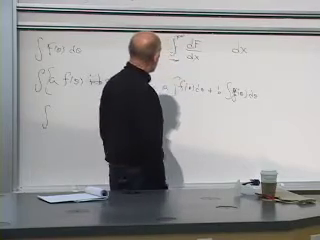
\includegraphics[width=0.88\textwidth]{lecture_06_figure_05.png}
\lectureframe{01:26:31.594}
\caption{Обычный прототип интегрирования Березина: интеграл от полной производной сводится к значениям на концах и обращается в нуль, когда функция затухает. Нижняя строка на доске частично закрыта, поэтому аккуратное уравнение приведено в тексте.}
\end{figure}

Мы хотим, чтобы интеграл по грассмановой переменной был линейным и обладал полезным свойством: интеграл от полной производной равен нулю. Для одной нечетной координаты потребуем
\begin{align}
\int d\theta\,[af(\theta)+bg(\theta)]
&=
a\int d\theta\,f(\theta)
+b\int d\theta\,g(\theta),\\
\int d\theta\,\partial_\theta f(\theta)&=0.
\end{align}
Второе условие — алгебраический аналог трансляционной инвариантности меры. У числовой прямой для нечетной координаты нет концов и нет суммирования по малым интервалам.

\begin{classroomqa}
\audiencequestion{Если неопределённого интеграла по грассмановой переменной нет, отказываемся ли мы тогда от идеи, что интегрирование является обратной операцией к дифференцированию? \lecturetimestamp{01:21:19}}
\lecturerresponse{Да. Интегрирование Березина — это определённый линейный функционал, а не операция взятия первообразной. Для одной грассмановой переменной оно фактически задаётся той же алгебраической операцией, что и дифференцирование.}
\end{classroomqa}

\begin{classroomqa}
\audiencequestion{Является ли интегрирование \(d^4x\) по всему пространству-времени тоже определённым интегралом? \lecturetimestamp{01:21:34}}
\lecturerresponse{Да. При интегрировании действия по пространству-времени граничные условия подразумеваются. Разница в том, что обычное интегрирование по пространству-времени можно понимать как предел сумм, тогда как грассманово интегрирование определяется алгебраически своим действием на конечный базис \(1,\theta\).}
\end{classroomqa}

\subsection{Одна переменная}

Любую функцию одной нечетной переменной можно записать так, чтобы коэффициент стоял справа, в фиксированном порядке,
\begin{equation}
f(\theta)=a+\theta b.
\end{equation}
Поскольку \(\partial_\theta\theta=1\), из правила для полной производной следует
\begin{equation}
\int d\theta\,1=0.
\end{equation}
Оставшуюся нормировку выбирают равной
\begin{equation}
\int d\theta\,\theta=1.
\end{equation}
Следовательно,
\begin{equation}
\int d\theta\,f(\theta)=b.
\end{equation}
Интеграл выделяет коэффициент при наивысшей возможной степени. При используемом здесь соглашении о левой производной
\begin{equation}
\partial_\theta f=b
=\int d\theta\,f.
\end{equation}

\begin{classroomqa}
\audiencequestion{Существует ли функция \(F(\theta)\), удовлетворяющая условию \(\partial_\theta F=\theta\)? \lecturetimestamp{01:30:05}}
\lecturerresponse{Нет. Такой функции понадобился бы член, пропорциональный \(\theta^2\), но \(\theta^2=0\). Это ещё один способ увидеть, почему не существует грассманова аналога неопределённой первообразной.}
\end{classroomqa}

\subsection{Две переменные и порядок меры}

Для комплексной пары \(\theta,\bar\theta\) запишем общую чётную функцию в упорядоченной форме
\begin{equation}
f(\theta,\bar\theta)
=a+\bar\theta\psi+\bar\psi\theta+b\,\bar\theta\theta.
\end{equation}
Членов более высокой степени нет, поскольку
\begin{equation}
\theta^2=\bar\theta^2=0,
\qquad
\bar\theta\theta=-\theta\bar\theta.
\end{equation}

Теперь зафиксируем соглашение
\begin{equation}
\int d\theta\,d\bar\theta\,
\bar\theta\theta=1.
\end{equation}
В повторных интегралах первой действует соседняя операция \(d\bar\theta\). Тогда таблица такова:
\begin{align}
\int d\theta\,d\bar\theta\,1&=0,\\
\int d\theta\,d\bar\theta\,\theta&=0,\\
\int d\theta\,d\bar\theta\,\bar\theta&=0,\\
\int d\theta\,d\bar\theta\,\bar\theta\theta&=1.
\end{align}
Тем самым
\begin{equation}
\int d\theta\,d\bar\theta\,
f(\theta,\bar\theta)=b.
\end{equation}

\begin{classroomqa}
\audiencequestion{Для члена, линейного по \(\theta\), неужели именно интегрирование по \(\theta\) обращает двойной интеграл в нуль? \lecturetimestamp{01:34:59}}
\lecturerresponse{Нет; в устном объяснении роли были перепутаны. Интегрирование \(\theta\) по \(\theta\) даёт единицу. Тогда результат уже не содержит \(\bar\theta\), и оставшийся интеграл по \(\bar\theta\) от единицы равен нулю. В любом случае двойной интеграл даёт ненулевой результат только тогда, когда присутствуют обе переменные.}
\end{classroomqa}

\begin{classroomqa}
\audiencequestion{Если \(\theta\) и \(\bar\theta\) переставить, меняет ли интеграл знак? \lecturetimestamp{01:36:33}}
\lecturerresponse{Да. Нечётные переменные и нечётные меры антикоммутируют. При соглашении выше
\[
\int d\bar\theta\,d\theta\,\bar\theta\theta=-1.
\]
Поэтому нужно выбрать порядок и затем последовательно его сохранять. Физика не зависит от соглашения, но промежуточные знаки зависят.}
\end{classroomqa}

Для \(n\) независимых грассмановых переменных схема сразу ясна:
\begin{equation}
\int d\theta_n\cdots d\theta_1\,
f(\theta_1,\ldots,\theta_n)
\end{equation}
выделяет коэффициент при упорядоченном старшем мономе \(\theta_1\cdots\theta_n\) с точностью до знака, фиксированного выбранным порядком переменных и мер. Это простое правило выделения компонент лежит в основе действий в суперпространстве. Вариация суперсимметрии превращается в нечётную полную производную, и интеграл по суперпространству отбрасывает её, точно так же как обычное действие отбрасывает полную производную по пространству-времени при подходящих граничных условиях.

\section{Почему столь малое исчисление обладает такой силой}

Правила выглядят почти тривиально:
\begin{equation}
\int d\theta\,1=0,
\qquad
\int d\theta\,\theta=1.
\end{equation}
И всё же они позволяют строить теории поля с взаимодействием, в которых соотношения между бозонными и фермионными массами и константами связи автоматически сохраняются. Назначение исчисления суперпространства то же, что и назначение тензорного исчисления в теории относительности: организовать обозначения так, чтобы нужная симметрия сохранялась при любых допустимых манипуляциях.

Ценой за это является тщательный учёт знаков. Каждая перестановка двух нечётных объектов вносит минус, и вычисление может быть концептуально правильным, но дать сбой из-за одного выбора порядка. Эта трудность не декоративна; это алгебраическая тень фермионной статистики.

\begin{classroomqa}
\audiencequestion{Числа Грассмана были введены вместе с суперсимметрией или существовали раньше? \lecturetimestamp{01:41:19}}
\lecturerresponse{Они намного старше. Герман Грассман разработал лежащую в основе внешнюю алгебру в XIX веке. В дифференциальных формах уже используются антикоммутирующие базисные элементы; квантовая теория поля XX века и суперсимметрия нашли для той же математики новую физическую роль.}
\end{classroomqa}

Теперь мы готовы к конкретным построениям. Суперполя собирают полные бозон-фермионные мультиплеты, производные в суперпространстве сохраняют алгебру, а интегрирование Березина извлекает компонентное действие. Следующая задача — применить этот аппарат в простейшей одномерной модели, а затем перенести его в теорию поля.
